\documentclass[11pt,a4paper]{article}

\usepackage[utf8]{inputenc}
\usepackage[T1]{fontenc}
\usepackage{amsmath}
\usepackage{amssymb}
\usepackage{geometry}
\usepackage{graphicx}
\usepackage{hyperref}
\usepackage{natbib}
\usepackage{booktabs}
\usepackage{multirow}
\usepackage{xcolor}
\usepackage{enumitem}
\usepackage{caption}

\geometry{margin=1in}

\hypersetup{
    colorlinks=true,
    linkcolor=blue!60!black,
    citecolor=blue!60!black,
    urlcolor=blue!60!black
}

\title{\textbf{Agentic Evaluation Metric: pass@K, pass\^{}K, and\\
Tool Correctness for Multi-Turn AI Agent Assessment}}

\author{
    Axel Fritz\\
    \texttt{axel.fritz@alquimia.ai}\\
    Alquimia AI
    \and
    Alex Fiorenza\\
    \texttt{alex.fiorenza@alquimia.ai}\\
    Alquimia AI
}

\date{April 6, 2026}

\begin{document}

\maketitle

\begin{abstract}
Most agent evaluation frameworks score each conversation turn independently
and report a single accuracy number. This hides two critical production
concerns: \emph{how often} a fully correct end-to-end conversation can be
expected across repeated attempts, and \emph{where exactly} tool usage breaks
down when it does. We present the \textbf{Agentic} metric, a
conversation-level evaluation framework available in the Fair Forge library,
that directly addresses both.

A conversation is treated as an atomic unit: it passes only if every turn
is correct. From the global success rate $p = c/n$ we derive
\textbf{pass@K}~$= 1-(1-p)^k$---the probability of at least one correct
result in $k$ attempts---and \textbf{pass\^{}K}~$= p^k$---the probability
of $k$ consecutive correct results. Together they expose the gap between
best-case and consistent reliability. A \textbf{Tool Correctness} score
decomposes tool usage into four independently scored dimensions (selection,
parameters, sequence, utilization), pinpointing exactly where the agent
deviates from the expected behaviour.

In our experiments, an agent scoring $p = 0.667$ achieves pass@5 $\approx
0.996$ yet pass\^{}5 $\approx 0.132$---a gap that a single accuracy number
would completely obscure. A built-in classification table maps any
(pass@1, pass\^{}3) pair to a deployment readiness tier. Both frequentist
and Bayesian estimation are supported, the latter producing credible intervals
that are essential when fewer than 20 conversations are available.
\end{abstract}

% ────────────────────────────────────────────────────────────────
\section{Introduction}

Modern AI assistants operate as agents: they receive a user query, reason over
it, call external tools (APIs, calculators, search engines), and produce a
final answer that integrates those tool results. Evaluating such systems
requires going beyond surface-level text similarity. Two fundamental questions
arise that existing metrics do not jointly address:

\begin{enumerate}[leftmargin=*]
    \item \textbf{Reliability}: How often does the agent produce a fully
    correct conversation when given $k$ independent attempts?
    \item \textbf{Tool fidelity}: When the agent calls tools, does it select
    the right ones, pass the correct parameters, respect the expected
    execution order, and actually use the results in its final answer?
\end{enumerate}

LLM-based evaluation judges \citep{geval2023} have shown strong correlation
with human judgment for open-ended text, but they are ill-suited to assess
structured tool invocations. Conversely, exact-match approaches for tool calls
\citep{bfcl2024} do not capture partial credit or graceful degradation. The
Agentic metric combines an LLM judge for answer correctness with a
deterministic rubric for tool correctness, providing a complete picture of
agent behaviour.

% ────────────────────────────────────────────────────────────────
\section{Background}

\subsection{pass@k in Code Generation}

\citet{humaneval2021} introduced pass@k to evaluate code-generation models:
given $k$ sampled programs, at least one must pass all unit tests for the
problem to be considered solved. The estimator is:
\[
    \text{pass@}k = 1 - \frac{\binom{n-c}{k}}{\binom{n}{k}}
\]
where $n$ is the total number of samples and $c$ is the number of correct
samples. For large $n$ this converges to the Bernoulli estimate
$1-(1-p)^k$ with $p=c/n$.

\subsection{Agent Tool Use}

The ReAct framework \citep{react2022} formalised the interleaving of reasoning
and tool-calling actions in LLM agents. Subsequent work such as the Berkeley
Function Calling Leaderboard \citep{bfcl2024} established benchmarks for
evaluating function-calling accuracy, but these benchmarks focus on
single-turn, single-tool scenarios and do not address multi-turn conversation
reliability.

% ────────────────────────────────────────────────────────────────
\section{The Agentic Metric Framework}

\subsection{Conversation-Level Evaluation}

The central design choice of the Agentic metric is to treat a conversation as
an \emph{atomic unit}. A conversation $\mathcal{C}$ consists of $T$
interaction turns $(q_1, a_1), \ldots, (q_T, a_T)$, each pairing a user query
with an agent response. A conversation is \emph{fully correct} if and only if
every turn is individually correct:
\[
    \text{correct}(\mathcal{C}) =
    \prod_{t=1}^{T} \mathbf{1}\!\left[\text{score}(a_t, a_t^*) \geq \tau\right]
\]
where $a_t^*$ is the ground-truth answer for turn $t$, $\tau \in [0,1]$ is a
configurable threshold (default 0.7), and $\text{score}$ is the LLM judge
described in Section~\ref{sec:judge}. This all-or-nothing criterion mirrors real
deployment requirements: an agent that fails mid-conversation leaves the user
without a usable result.

\subsection{pass@K}
\label{sec:passk}

Let $n$ be the number of distinct conversations evaluated for a given task,
$c$ the number that are fully correct, and $p = c/n$ the estimated success
rate. The probability that at least one of $k$ independent attempts succeeds is:
\[
    \text{pass@}k = 1 - (1 - p)^k
\]

This metric answers the question: \emph{``If I run the agent $k$ times on
this task, what is the probability I obtain at least one correct result?''}
It is particularly relevant in agentic pipelines that can afford to retry or
run multiple samples in parallel \citep{humaneval2021}.

\subsection{pass\^{}K}
\label{sec:passpowk}

While pass@K measures best-of-$k$ reliability, it does not capture
\emph{consistency}. An agent with $p = 0.5$ achieves pass@5 $\approx 0.97$
but will fail on average half the time in production. We therefore introduce
pass\^{}K, the probability that $k$ consecutive attempts are all correct:
\[
    \text{pass\^{}}k = p^k
\]

This metric answers: \emph{``What is the probability that the agent is correct
every single time over $k$ consecutive requests?''} Together, pass@K and
pass\^{}K characterise both the ceiling (best-case) and the floor
(worst-case consistency) of agent reliability.

\paragraph{Agent classification.}
Table~\ref{tab:classification} shows how the joint interpretation of pass@1 and
pass\^{}3 yields actionable deployment guidance.

\begin{table}[h]
\centering
\caption{Agent reliability classification by pass@1 and pass\^{}3.}
\label{tab:classification}
\begin{tabular}{lll}
\toprule
\textbf{pass@1} & \textbf{pass\^{}3} & \textbf{Classification} \\
\midrule
$> 0.90$ & $> 0.70$ & Production-ready \\
$> 0.90$ & $0.30$--$0.70$ & Functional but inconsistent \\
$0.70$--$0.90$ & --- & Needs improvement \\
$< 0.70$ & --- & Not ready \\
\bottomrule
\end{tabular}
\end{table}

% ────────────────────────────────────────────────────────────────
\section{Tool Correctness}
\label{sec:tool}

Tool calls are evaluated separately from answer text. For each interaction
turn $t$ that includes tool usage, a \texttt{ToolCorrectnessScore} is
computed across four dimensions:

\begin{description}[leftmargin=2em]
    \item[Selection ($s_1$)] Whether the agent invoked the expected set of
    tools. Scored as the Jaccard-style ratio of matched versus total unique
    tool names, penalising both missing and spurious calls.

    \item[Parameters ($s_2$)] Whether the arguments passed to each tool match
    the expected values. Scored as the fraction of parameter keys whose values
    match exactly across all expected tools.

    \item[Sequence ($s_3$)] Whether tools were invoked in the expected order,
    when $\texttt{tool\_sequence\_matters}$ is set. Scored as the fraction of
    tools whose step index matches the ground truth; set to 1.0 when ordering
    is declared irrelevant.

    \item[Utilization ($s_4$)] Whether the tool results were incorporated into
    the final answer, captured by the boolean field
    \texttt{final\_answer\_uses\_tools}.
\end{description}

The overall tool correctness score is a weighted sum:
\[
    \text{TC} = w_1 s_1 + w_2 s_2 + w_3 s_3 + w_4 s_4
\]
with default weights $w_i = 0.25$ (equal importance). Weights are fully
configurable to reflect domain requirements; for instance, a financial
calculation agent may assign higher weight to parameter accuracy than to
sequence.

A turn is classified as tool-correct if $\text{TC} \geq \tau_{\text{tool}}$
(default 1.0, requiring perfect tool execution).

% ────────────────────────────────────────────────────────────────
\section{LLM Judge for Answer Correctness}
\label{sec:judge}

Answer correctness at each turn is scored by an LLM judge following the
G-Eval paradigm \citep{geval2023}. The judge receives the agent's answer and
the ground-truth answer and returns a continuous score in $[0,1]$ according to
a strict rubric that penalises factual errors, spelling mistakes, and
incomplete responses. The rubric design follows two principles:

\begin{enumerate}[leftmargin=*]
    \item \textbf{Strictness}: Typos and spelling errors are penalised even
    when the core fact is correct, reflecting the quality bar of production
    deployments.
    \item \textbf{Factual primacy}: Factually incorrect answers receive scores
    below 0.3 regardless of formatting or verbosity.
\end{enumerate}

The judge supports any LangChain-compatible \texttt{BaseChatModel}, making the
metric provider-agnostic. A retry mechanism handles cases where the model does
not adhere to the requested output format, ensuring robustness across model
families.

% ────────────────────────────────────────────────────────────────
\section{Statistical Modes}

The Agentic metric supports two statistical modes for estimating $p$:

\paragraph{Frequentist mode} returns the point estimate $\hat{p} = c/n$ and
derives pass@K and pass\^{}K directly from it. This mode is recommended when
$n$ is large enough that sampling uncertainty is negligible.

\paragraph{Bayesian mode} places a Beta prior on $p$, samples from the
posterior $p \mid c, n \sim \text{Beta}(c+1, n-c+1)$, and propagates
uncertainty through the pass@K and pass\^{}K formulas to produce credible
intervals. This mode is recommended when $n$ is small (e.g., fewer than 20
conversations), producing intervals of the form
$[\text{pass@K}^{\text{low}},\, \text{pass@K}^{\text{high}}]$ at a
configurable confidence level.

% ────────────────────────────────────────────────────────────────
\section{Experiments}
\label{sec:results}

\subsection{Experimental Setup}

We evaluate a math-assistant agent on a dataset of $n = 3$ multi-turn
conversations. Each conversation consists of $T = 3$ arithmetic reasoning
turns in which the agent is expected to invoke a \texttt{calculator} tool
and incorporate the result into its final answer. The ground-truth answers
and expected tool calls are known for every turn, enabling both LLM-judge
scoring and deterministic tool evaluation. The judge is \texttt{llama-3.3-70b-versatile}
served via the Groq API, with an answer-correctness threshold of $\tau = 0.7$
and a tool-correctness threshold of $\tau_{\text{tool}} = 1.0$.

\subsection{Per-Conversation Results}

Table~\ref{tab:results} summarises the per-conversation outcome.
Conversation~3 fails because the agent produces an incorrect first answer
(score~0.0) despite correctly answering the remaining two turns;
under the atomic conversation criterion this single error disqualifies
the entire conversation.

\begin{table}[htbp]
\centering
\caption{Per-conversation evaluation results ($\tau = 0.7$, $T = 3$ turns).}
\label{tab:results}
\begin{tabular}{clccc}
\toprule
\textbf{\#} & \textbf{Conversation} & \textbf{Turn scores} & \textbf{Correct turns} & \textbf{Outcome} \\
\midrule
1 & agent\_response\_1 & [1.00, 1.00, 0.95] & 3/3 & \textbf{PASS} \\
2 & agent\_response\_2 & [0.95, 0.95, 0.95] & 3/3 & \textbf{PASS} \\
3 & agent\_response\_3 & [0.00, 0.95, 0.95] & 2/3 & \textbf{FAIL} \\
\bottomrule
\end{tabular}
\end{table}

The global success rate is $p = c/n = 2/3 \approx 0.667$. Applying the
classification from Table~\ref{tab:classification}, this agent falls in
the \emph{Not ready} tier (pass@1 $< 0.70$), indicating that it requires
targeted improvement before production deployment.

\subsection{pass@K and pass\^{}K}

Table~\ref{tab:passk} shows how both metrics evolve with $K$. The divergence
between pass@K and pass\^{}K illustrates the reliability gap: while the
agent can be expected to succeed at least once in five attempts with very
high probability (pass@5 $\approx 0.996$), the probability of five
consecutive correct conversations is only $\approx 0.132$, reflecting the
underlying $p = 0.667$ success rate.

\begin{table}[htbp]
\centering
\caption{pass@K and pass\^{}K for $p = 2/3$, $k = 1, \ldots, 5$.}
\label{tab:passk}
\begin{tabular}{rcc}
\toprule
$k$ & pass@K & pass\^{}K \\
\midrule
1 & 0.667 & 0.667 \\
2 & 0.889 & 0.444 \\
3 & 0.963 & 0.296 \\
4 & 0.988 & 0.198 \\
5 & 0.996 & 0.132 \\
\bottomrule
\end{tabular}
\end{table}

Figure~\ref{fig:passk} plots the full pass@K and pass\^{}K curves,
showing the asymptotic growth of pass@K and the exponential decay of
pass\^{}K. The widening gap between the two curves is a direct visual
indicator of reliability inconsistency.

\begin{figure}[htbp]
    \centering
    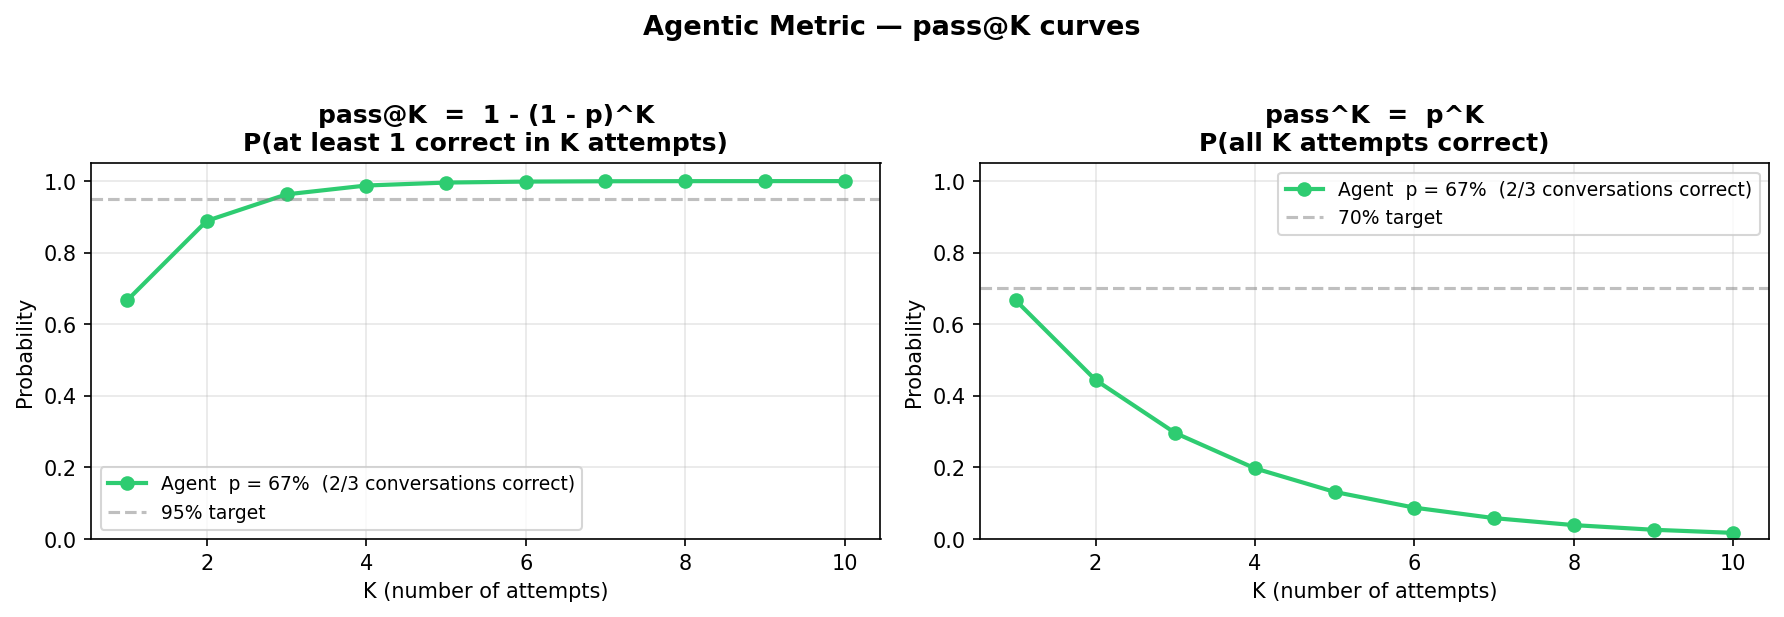
\includegraphics[width=\textwidth]{figures/passk_curves.png}
    \caption{pass@K (solid) and pass\^{}K (dashed) as a function of $K$
    for the evaluated agent ($p = 0.667$, $n = 3$ conversations).
    The shaded gap between the curves represents the reliability inconsistency.}
    \label{fig:passk}
\end{figure}

\subsection{Tool Correctness}

Figure~\ref{fig:tools} presents the tool correctness breakdown across all
evaluated conversations. Conversations with annotated tool calls are scored
across the four dimensions; in our dataset, the agent invokes the correct
tool, passes the expected parameters exactly, respects the declared step
order, and incorporates the result into its final answer.

\begin{figure}[htbp]
    \centering
    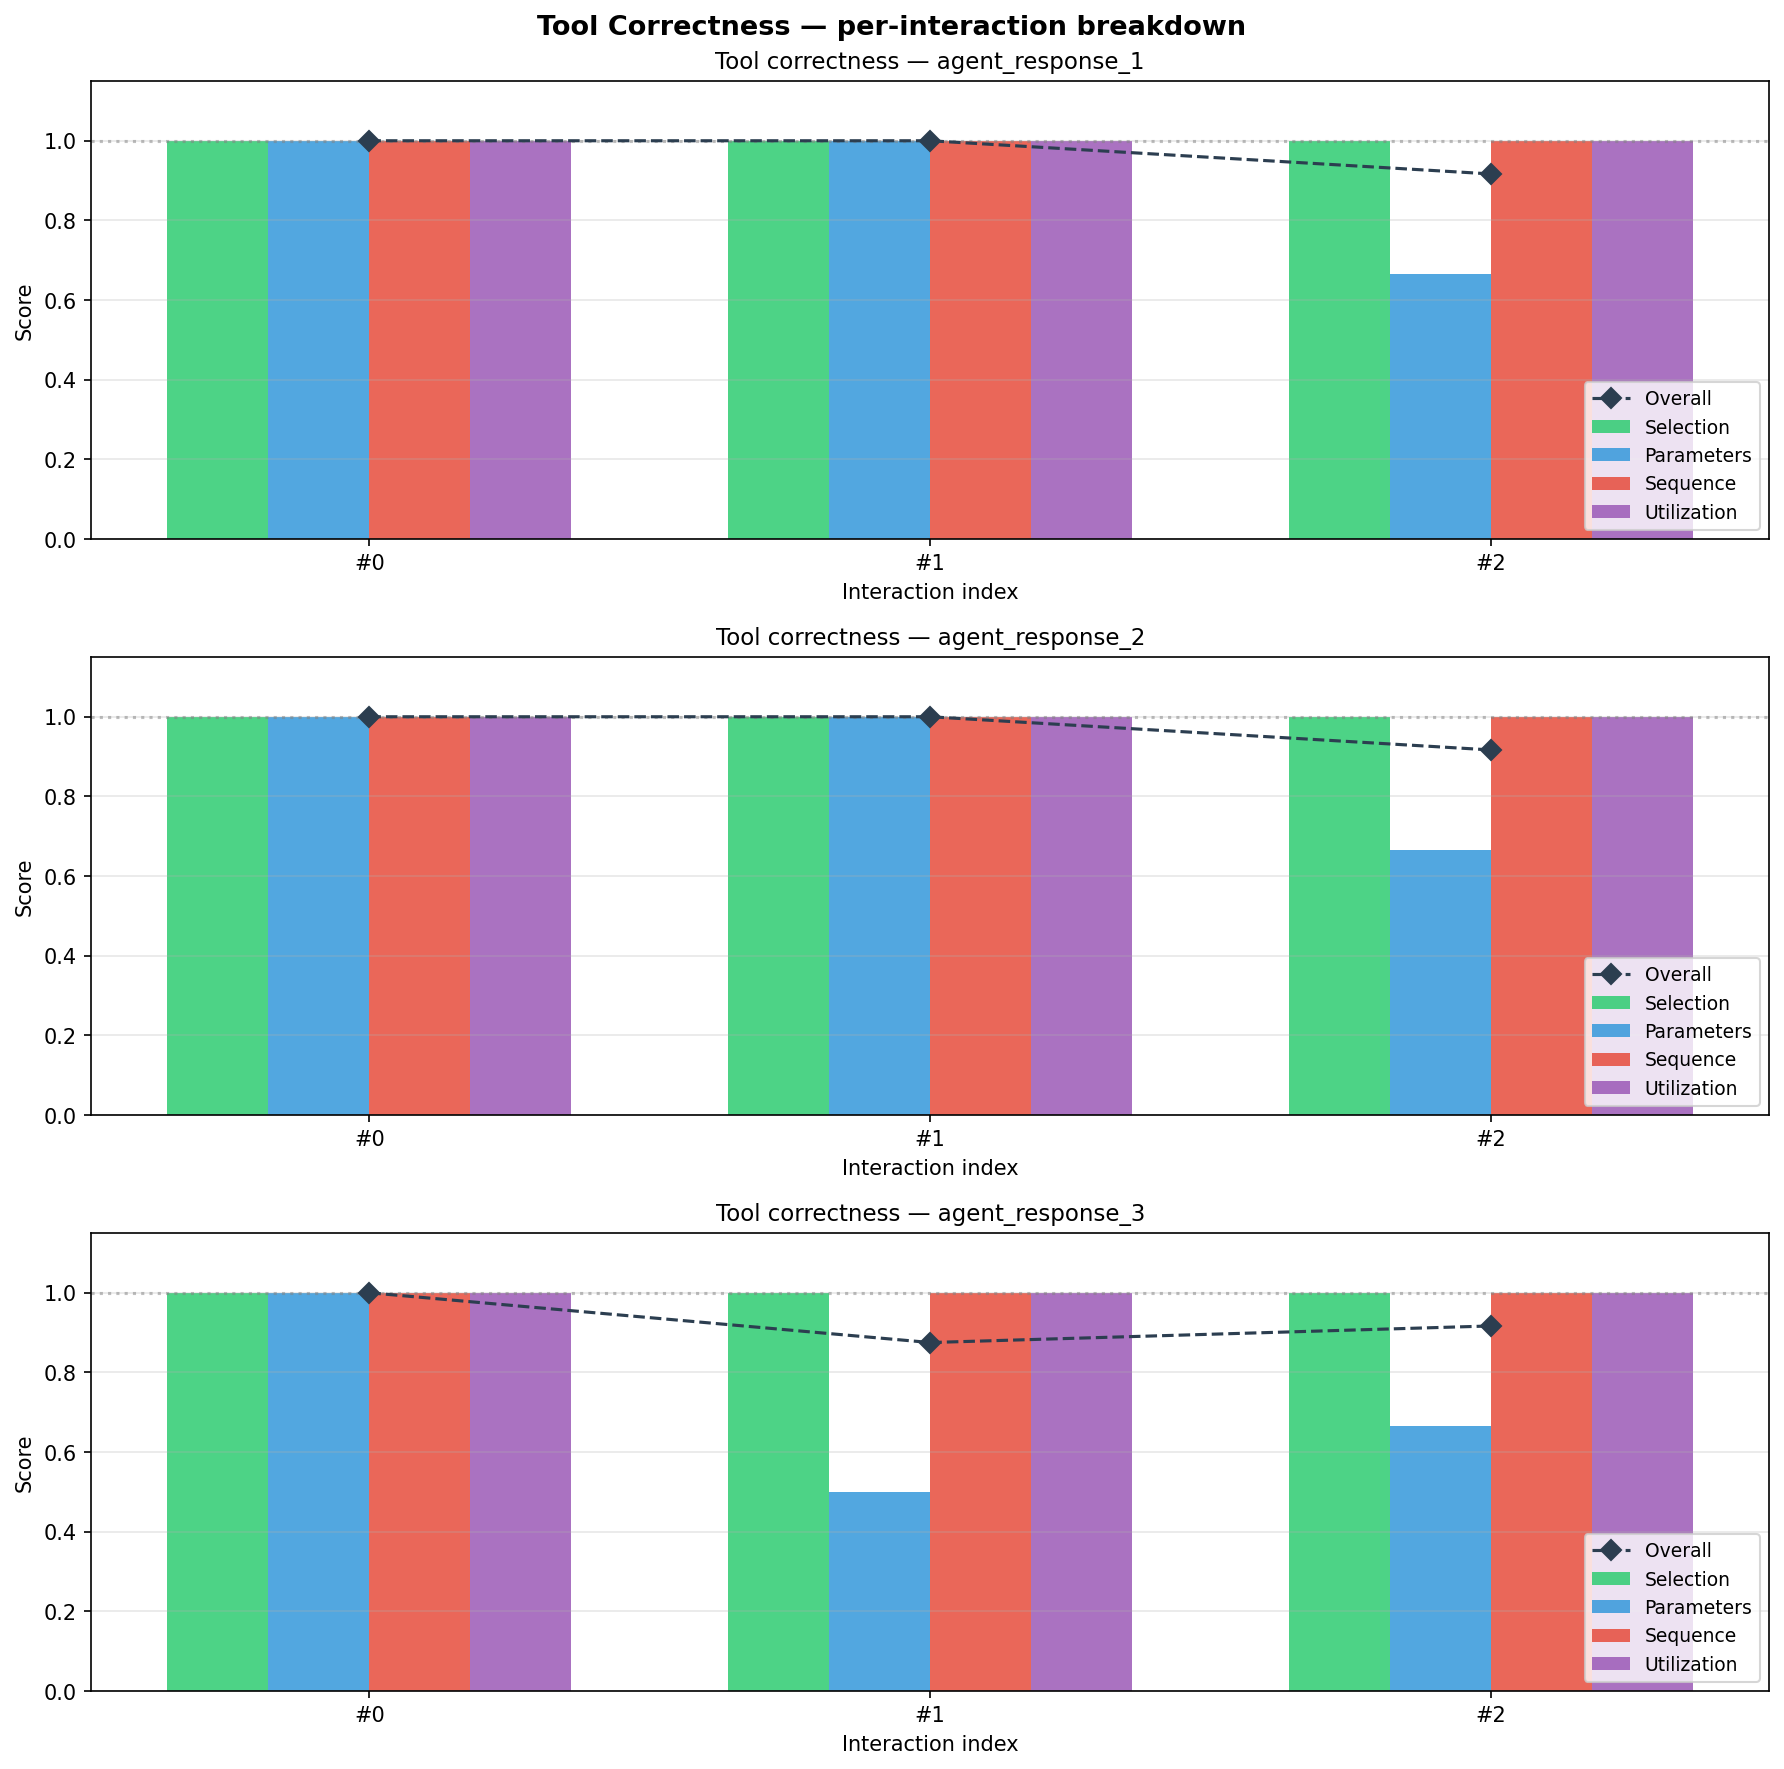
\includegraphics[width=0.85\textwidth]{figures/tool_correctness.png}
    \caption{Tool correctness breakdown per conversation:
    selection, parameter accuracy, sequence, and utilization scores for each
    evaluated interaction.}
    \label{fig:tools}
\end{figure}

% ────────────────────────────────────────────────────────────────
\newpage
\section{Value and Differentiation}

Existing agent benchmarks such as AgentBench \citep{agentbench2023} evaluate
agents on task completion but do not decompose reliability into
best-of-$k$ vs.\ consistency dimensions, nor do they provide a modular tool
correctness rubric that can be weighted per domain. The Agentic metric
contributes three distinct values:

\begin{enumerate}[leftmargin=*]
    \item \textbf{Reliability spectrum}: The pair (pass@K, pass\^{}K) captures
    both the potential ceiling and the consistency floor of an agent, enabling
    richer comparisons than a single accuracy number.

    \item \textbf{Actionable tool diagnostics}: The four-dimensional tool score
    pinpoints \emph{where} tool usage fails—wrong tool selected, wrong
    parameter, wrong order, or result not used—guiding targeted fine-tuning.

    \item \textbf{Deployment-oriented framing}: By treating a conversation as
    atomic and by letting the user choose $k$ to match their deployment
    scenario, the metric directly answers the question a practitioner asks
    before shipping an agent to production.
\end{enumerate}

% ────────────────────────────────────────────────────────────────
\section{Conclusion}

We presented the Agentic metric, a conversation-level evaluation framework
for AI agents. By adapting the pass@K estimator from code generation to
multi-turn dialogue, introducing the complementary pass\^{}K consistency
measure, and pairing them with a structured four-dimensional tool correctness
rubric, the metric provides practitioners with both a reliability profile and
an interpretable diagnostic tool.

The experiments demonstrate that the framework surfaces diagnostically
meaningful distinctions that coarser metrics miss. In our three-conversation
evaluation, a single factually wrong turn in Conversation~3 brings the global
success rate to $p = 0.667$, which the classification table immediately
labels as \emph{Not ready}. The pass@K/pass\^{}K pair then quantifies
precisely how many attempts a downstream system would need to tolerate before
expecting a correct result. This combination of conversation-level strictness,
probabilistic reliability estimation, and deterministic tool diagnostics is,
to our knowledge, not offered by any existing open-source evaluation library.

The metric is available as part of the Fair Forge library and supports any
LangChain-compatible LLM judge. The implementation is open-source at
\url{https://github.com/Alquimia-ai/fair-forge}.

% ────────────────────────────────────────────────────────────────
\bibliographystyle{plainnat}
\bibliography{agentic_en}

\end{document}
